\documentclass[a4paper, 11pt]{article}
\author{Kajetan Kaczmarek}
\usepackage{amsmath}
\usepackage{graphicx}
\usepackage{listings}
\usepackage[T1]{fontenc}
\usepackage[utf8]{inputenc}
\usepackage{breqn}
\usepackage[polish]{babel}
\usepackage{color} %red, green, blue, yellow, cyan, magenta, black, white
\definecolor{mygreen}{RGB}{28,172,0} % color values Red, Green, Blue
\definecolor{mylilas}{RGB}{170,55,241}
\graphicspath{ {./} }


\lstset{language=Matlab,%
    basicstyle=\tiny,
    breaklines=true,%
    morekeywords={matlab2tikz},
    keywordstyle=\color{blue},%
    morekeywords=[2]{1}, keywordstyle=[2]{\color{black}},
    identifierstyle=\color{black},%
    stringstyle=\color{mylilas},
    commentstyle=\color{mygreen},%
    showstringspaces=false,%without this there will be a symbol in the places where there is a space
    numbers=left,%
    numberstyle={\tiny \color{black}},% size of the numbers
    numbersep=9pt, % this defines how far the numbers are from the text
    emph=[1]{for,end,break},emphstyle=[1]\color{red}, %some words to emphasise
    %emph=[2]{word1,word2}, emphstyle=[2]{style},    
}

\begin{document}
\title{Sprawozdanie STP \\* Projekt nr.1 \\* 
Zadanie 9 \\*}
\maketitle
\begin{enumerate}
\item Wyznaczanie modeli transmitancji \\*
Do wyznaczenia modeli użyłem programu : 
\lstinputlisting{STP_P_1Modele.m}
Po wymnożeniu transmitancja ma postać 
\begin{center} \[ G(s) = \dfrac{(s + 1)(s + 9)}{(s + 10)(s + 11)(s + 12)} = \dfrac{s^2 + 10s + 9}{s^3 + 33s^2 + 362s + 1320} = \dfrac{s^{-1} + 10s^{-2} + 9s^{-3}}{1 + 33s^{-1} + 362s^{-2} + 1320s^{-3}} \]
\end{center}
Czyli macierze dla wariantu pierwszego wyglądają następująco:
 \[ A = 	
 \begin{bmatrix}
   -33 & -362 & -1320\\
   1 & 0 & 0\\
   0 & 1 & 0
  \end{bmatrix}
B = 
\begin{bmatrix}
	1 \\
	0 \\
	0 \\
\end{bmatrix}
C = 
\begin{bmatrix}
	1 & 10 & 9 \\
\end{bmatrix}
D = \begin{bmatrix}
0 \end{bmatrix}
 \]
Reprezentacja graficzna : 
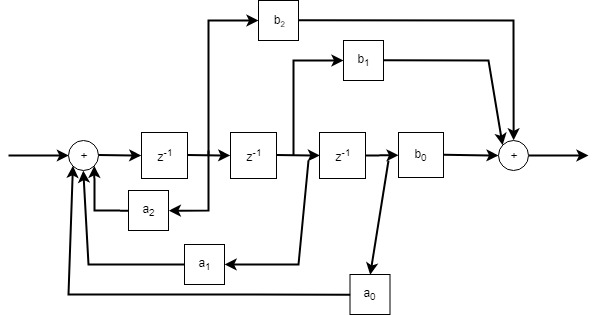
\includegraphics[scale=0.5]{Wariant1.jpg}
Oraz dla wartiantu drugiego:

 \[ A = 	
 \begin{bmatrix}
   -33 & 1 & 0 \\
   -362 & 0 & 1\\
   -1320 & 0 & 0
  \end{bmatrix}
B = 
\begin{bmatrix}
	1 \\
	10 \\
	9 \\
\end{bmatrix}
C = 
\begin{bmatrix}
	1 & 0 & 0 \\
\end{bmatrix}
D = \begin{bmatrix}
0 \end{bmatrix}
\]
Reprezentacja graficzna : 
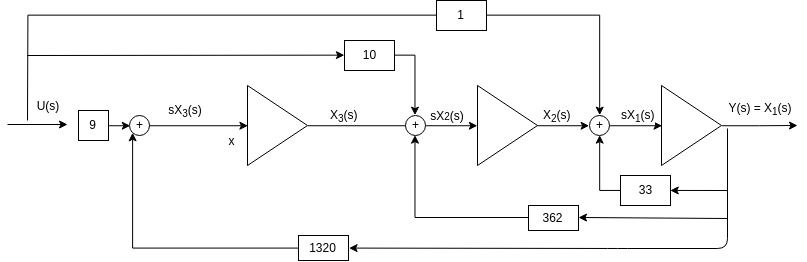
\includegraphics{Wariant2.jpg}
\end{enumerate}
\end{document}
